\section{Basics}

Vectors are denoted by boldface letters such as $\mathbf{A}$. In Cartesian coordinates any vector can be written as
\begin{equation}
    \mathbf{A} = A_x \mathbf{e}_x + A_y \mathbf{e}_y + A_z \mathbf{e}_z,
\end{equation}
and its magnitude is
\begin{equation}
    |\mathbf{A}| = \sqrt{A_x^2 + A_y^2 + A_z^2}.
\end{equation}

\subsection{Scalars and scaling}
A scalar is a quantity described only by magnitude (e.g. temperature, mass, charge). Multiplying a vector by a scalar scales its magnitude; a negative scalar reverses its direction:
\begin{equation}
    \alpha\mathbf{A}=\alpha A_x \mathbf{e}_x+\alpha A_y \mathbf{e}_y+\alpha A_z \mathbf{e}_z.
\end{equation}

\subsection{Addition and subtraction}
Vector addition and subtraction are performed componentwise:
\begin{equation}
    \mathbf{A}\pm\mathbf{B}=(A_x\pm B_x)\mathbf{e}_x+(A_y\pm B_y)\mathbf{e}_y+(A_z\pm B_z)\mathbf{e}_z.
\end{equation}
Geometrically, addition corresponds to the parallelogram rule; subtraction can be viewed by placing vectors head-to-tail so that $\mathbf{B}-\mathbf{A}$ is the vector from the tip of $\mathbf{A}$ to the tip of $\mathbf{B}$.

\begin{figure}[H]
    \centering
    
\includegraphics[width=0.6\textwidth]{figures/vec_sum_diff.png}
    \caption{Vector addition (parallelogram) and subtraction (head-to-tail).}
    \label{fig:vec_sum_diff}
\end{figure}

\begin{example}[Vector addition and subtraction]
Given
\begin{equation}
\mathbf{A}=4\mathbf{e}_x+4\mathbf{e}_y,
\qquad
\mathbf{B}=\mathbf{e}_x+8\mathbf{e}_y.
\end{equation}
Find the sum and difference and their magnitudes.

By componentwise addition,
\begin{equation}
\mathbf{S}=\mathbf{A}+\mathbf{B}=(4+1)\mathbf{e}_x+(4+8)\mathbf{e}_y=5\mathbf{e}_x+12\mathbf{e}_y,
\end{equation}
so
\begin{equation}
|\mathbf{S}|=\sqrt{5^2+12^2}=\sqrt{25+144}=\sqrt{169}=13.
\end{equation}
For the difference,
\begin{equation}
\mathbf{D}=\mathbf{B}-\mathbf{A}=(1-4)\mathbf{e}_x+(8-4)\mathbf{e}_y=-3\mathbf{e}_x+4\mathbf{e}_y,
\end{equation}
hence
\begin{equation}
|\mathbf{D}|=\sqrt{(-3)^2+4^2}=\sqrt{9+16}=\sqrt{25}=5.
\end{equation}
\end{example}

\subsection{Dot product}
The dot (scalar) product of two vectors is a scalar defined by
\begin{equation}
    \mathbf{A}\cdot\mathbf{B}=|\mathbf{A}|\,|\mathbf{B}|\cos\theta,
\end{equation}
where $\theta$ is the angle between them. In components,
\begin{equation}
    \mathbf{A}\cdot\mathbf{B}=A_xB_x+A_yB_y+A_zB_z.
\end{equation}

\begin{figure}[H]
    \centering
    
\includegraphics[width=0.5\textwidth]{figures/vec_dot_product.png}
    \caption{Dot product: projection and angle $\theta$.}
    \label{fig:vec_dot}
\end{figure}

\begin{example}[Angle from the dot product]
Given
\begin{equation}
\mathbf{A}=\sqrt{3}\,\mathbf{e}_x+\mathbf{e}_y,
\qquad
\mathbf{B}=2\mathbf{e}_x,
\end{equation}
find the angle $\theta$ between the two vectors.

First compute magnitudes:
\begin{equation}
|\mathbf{A}|=\sqrt{(\sqrt{3})^2+1^2}=2,
\qquad
|\mathbf{B}|=\sqrt{2^2}=2.
\end{equation}
Then compute the dot product:
\begin{equation}
\mathbf{A}\cdot\mathbf{B}=A_xB_x+A_yB_y=(\sqrt{3})(2)+1\cdot 0=2\sqrt{3}.
\end{equation}
Using $\mathbf{A}\cdot\mathbf{B}=|\mathbf{A}|\,|\mathbf{B}|\cos\theta$,
\begin{equation}
2\sqrt{3}=2\cdot 2\cos\theta=4\cos\theta,
\qquad
\cos\theta=\frac{\sqrt{3}}{2},
\end{equation}
thus
\begin{equation}
\theta=\cos^{-1}\!\left(\frac{\sqrt{3}}{2}\right)=30^\circ.
\end{equation}
\end{example}

\begin{example}[Water molecule bond angle]
Dot products are frequently used in molecular geometry. Let the oxygen atom be at the origin, and let
\begin{equation}
\mathrm{H}_1=(0.757,\,0,\,0.586),
\qquad
\mathrm{H}_2=(-0.757,\,0,\,0.586)
\end{equation}
in the $xz$-plane (units: \AA). Define bond vectors $\mathbf{u}=\overrightarrow{\mathrm{OH}_1}$ and $\mathbf{v}=\overrightarrow{\mathrm{OH}_2}$. Then
\begin{equation}
\cos\alpha=\frac{\mathbf{u}\cdot\mathbf{v}}{|\mathbf{u}|\,|\mathbf{v}|}
=\frac{0.586^2-0.757^2}{0.757^2+0.586^2}\approx -0.251,
\end{equation}
so
\begin{equation}
\alpha=\arccos(-0.251)\approx 104.5^\circ.
\end{equation}
Equivalently, if $\mathbf{u}=(a,0,b)$ and $\mathbf{v}=(-a,0,b)$, then
\begin{equation}
\cos\alpha=\frac{b^2-a^2}{a^2+b^2}.
\end{equation}
\end{example}

\begin{figure}[H]
    \centering
    
\includegraphics[width=0.5\textwidth]{figures/vec_water_bond_angle.png}
    \caption{Water molecule bond angle from a dot-product calculation.}
    \label{fig:water_bond}
\end{figure}

\begin{example}[Orthogonality test via dot product]
Given
\begin{equation}
\mathbf{p}=2\mathbf{e}_x-\mathbf{e}_y+2\mathbf{e}_z,
\qquad
\mathbf{q}=\mathbf{e}_x+2\mathbf{e}_y,
\end{equation}
determine whether $\mathbf{p}$ and $\mathbf{q}$ are perpendicular.

Compute the dot product:
\begin{equation}
\mathbf{p}\cdot\mathbf{q}=2\cdot 1+(-1)\cdot 2+2\cdot 0=2-2+0=0.
\end{equation}
Therefore, $\mathbf{p}\perp\mathbf{q}$.
\end{example}

\subsection{Cross product}
The cross (vector) product $\mathbf{A}\times\mathbf{B}$ is a vector perpendicular to both $\mathbf{A}$ and $\mathbf{B}$, with magnitude
\begin{equation}
    |\mathbf{A}\times\mathbf{B}|=|\mathbf{A}|\,|\mathbf{B}|\sin\theta,
\end{equation}
and direction given by the right-hand rule. Componentwise it may be written as the determinant
\begin{equation}
    \mathbf{A}\times\mathbf{B}=\begin{vmatrix}\mathbf{e}_x & \mathbf{e}_y & \mathbf{e}_z \\\\ A_x & A_y & A_z \\\\ B_x & B_y & B_z \end{vmatrix}.
\end{equation}

\begin{figure}[H]
    \centering
    
\includegraphics[width=0.5\textwidth]{figures/vec_cross_product.png}
    \caption{Cross product: right-hand rule and parallelogram area.}
    \label{fig:vec_cross}
\end{figure}

\begin{example}[Cross product and unit normal vector]
Given
\begin{equation}
\mathbf{A}=-\mathbf{e}_x+\mathbf{e}_y+\mathbf{e}_z,
\qquad
\mathbf{B}=\mathbf{e}_x-\mathbf{e}_y+\mathbf{e}_z,
\end{equation}
find a unit vector $\mathbf{e}_n$ perpendicular to both vectors (right-hand orientation), and find the angle between $\mathbf{A}$ and $\mathbf{B}$.

First compute
\begin{equation}
\mathbf{A}\times\mathbf{B}=\begin{vmatrix}
\mathbf{e}_x&\mathbf{e}_y&\mathbf{e}_z\\
-1&1&1\\
1&-1&1
\end{vmatrix}
=2\mathbf{e}_x+2\mathbf{e}_y.
\end{equation}
Its magnitude is
\begin{equation}
|\mathbf{A}\times\mathbf{B}|=\sqrt{2^2+2^2}=2\sqrt{2},
\end{equation}
so the unit normal is
\begin{equation}
\mathbf{e}_n=\frac{\mathbf{A}\times\mathbf{B}}{|\mathbf{A}\times\mathbf{B}|}
=\frac{1}{\sqrt{2}}\left(\mathbf{e}_x+\mathbf{e}_y\right).
\end{equation}

For the angle, compute
\begin{equation}
\mathbf{A}\cdot\mathbf{B}=(-1)(1)+1(-1)+1(1)=-1,
\end{equation}
and
\begin{equation}
|\mathbf{A}|=\sqrt{3},
\qquad
|\mathbf{B}|=\sqrt{3}.
\end{equation}
Hence
\begin{equation}
\cos\theta=\frac{\mathbf{A}\cdot\mathbf{B}}{|\mathbf{A}|\,|\mathbf{B}|}=-\frac{1}{3},
\qquad
\theta=\cos^{-1}\!\left(-\frac{1}{3}\right)\approx 109.47^\circ.
\end{equation}
\end{example}

\subsection{Scalar triple product}
The scalar triple product $(\mathbf{A}\times\mathbf{B})\cdot\mathbf{C}$ equals the signed volume of the parallelepiped spanned by $\mathbf{A},\mathbf{B},\mathbf{C}$ and satisfies cyclic permutation symmetry.

\begin{equation}
(\mathbf{A}\times\mathbf{B})\cdot\mathbf{C}
=(\mathbf{B}\times\mathbf{C})\cdot\mathbf{A}
=(\mathbf{C}\times\mathbf{A})\cdot\mathbf{B}.
\end{equation}

\begin{figure}[H]
    \centering
    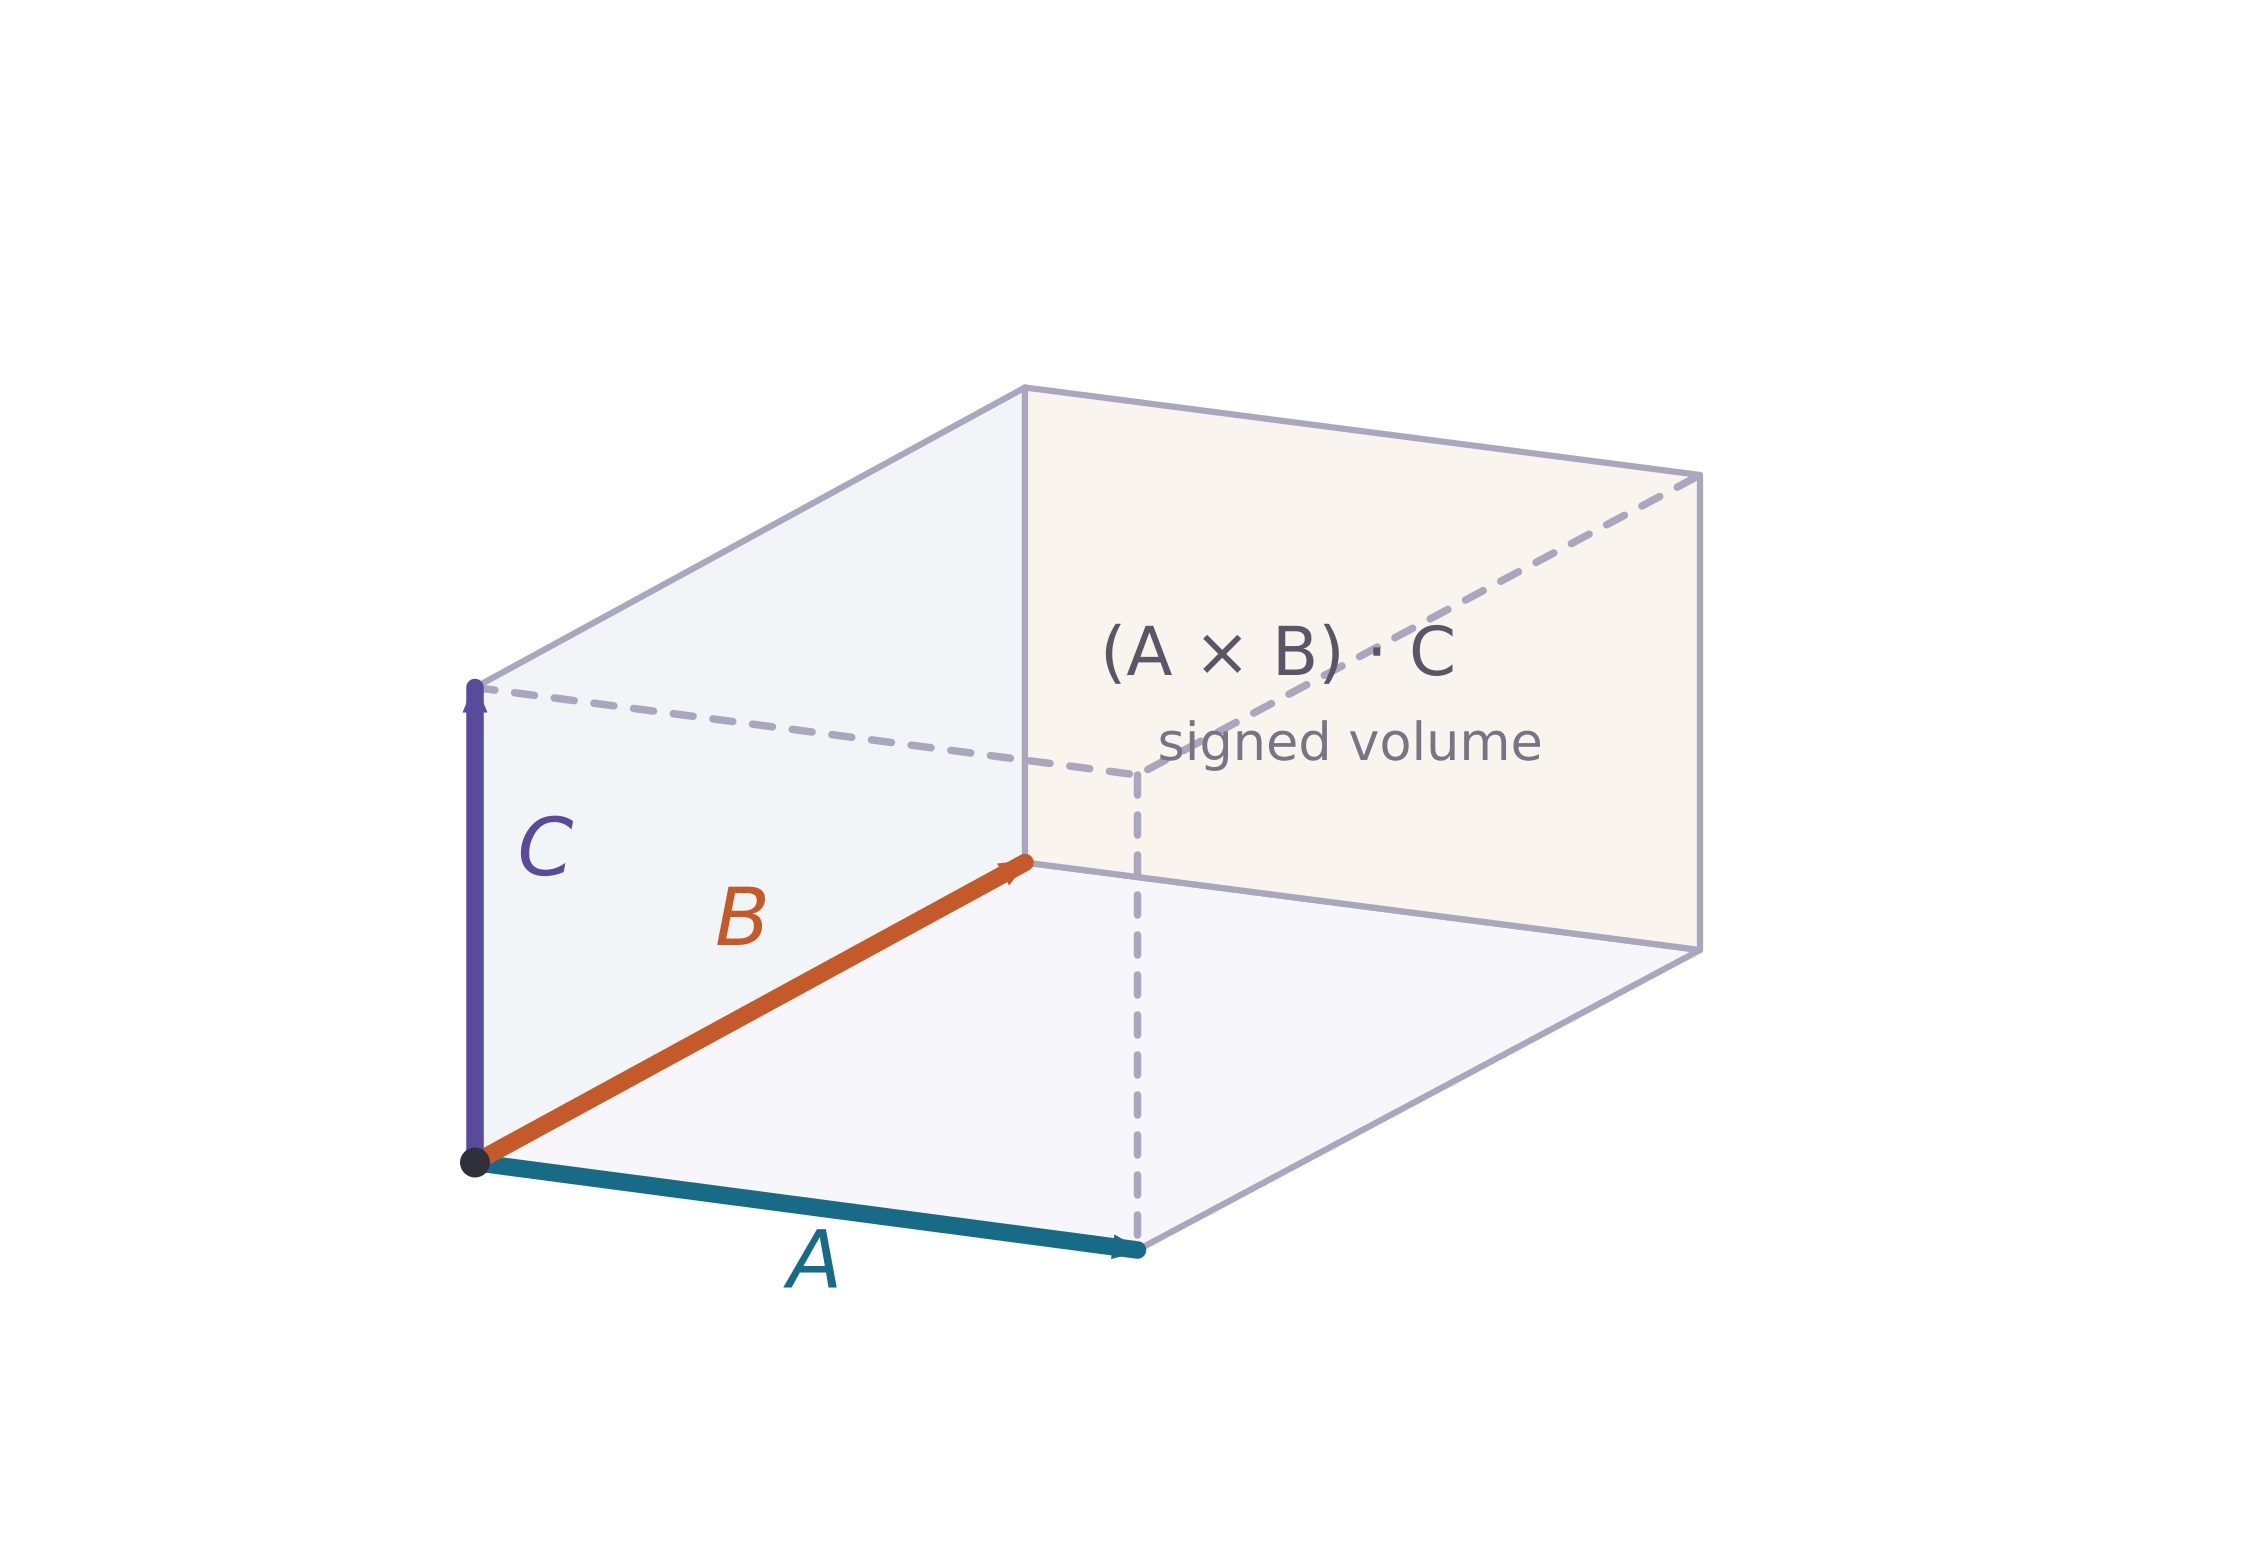
\includegraphics[width=0.5\textwidth]{figures/vec_scalar_triple_product.png}
    \caption{Scalar triple product as the signed volume of a parallelepiped.}
    \label{fig:scalar_triple_product}
\end{figure}

\begin{example}[Scalar triple product and volume]
Let
\begin{equation}
\mathbf{A}=\mathbf{e}_x+\mathbf{e}_y,
\qquad
\mathbf{B}=\mathbf{e}_y+\mathbf{e}_z,
\qquad
\mathbf{C}=\mathbf{e}_x+\mathbf{e}_z.
\end{equation}
Find $(\mathbf{A}\times\mathbf{B})\cdot\mathbf{C}$ and the corresponding volume.

First,
\begin{equation}
\mathbf{A}\times\mathbf{B}=
\begin{vmatrix}
\mathbf{e}_x & \mathbf{e}_y & \mathbf{e}_z \\
1 & 1 & 0 \\
0 & 1 & 1
\end{vmatrix}
=\mathbf{e}_x-\mathbf{e}_y+\mathbf{e}_z.
\end{equation}
Then
\begin{equation}
(\mathbf{A}\times\mathbf{B})\cdot\mathbf{C}
=(\mathbf{e}_x-\mathbf{e}_y+\mathbf{e}_z)\cdot(\mathbf{e}_x+\mathbf{e}_z)
=1+0+1=2.
\end{equation}
Hence the signed volume is $2$, and the geometric volume is $|2|=2$.
\end{example}

\begin{definition}
A definition is a precise statement of meaning.
\end{definition}
